% This document contains the notes we take during the project
\documentclass[report/main.tex]{subfiles}

\begin{document}
    \section{Db change}
        Did it first, got write denial, waited 
        
        did a second time 4.4 million rows, which crashed when we tried to transfer (too big) which made it even harder to transfer (SQL dump worked?!?!)

    \section{Password Hasher}
        Allowed old due to the setup
        
    \subsection{Monitoring}
        \label{SubSec:monitoring}
            % - How do you monitor your systems and what precisely do you monitor?
            \subsubsection{Setup}
                The monitoring of the EvilTwitter application was done using the monitoring and alerting toolkit Prometheus\footnote{\hyperlink{https://prometheus.io/}{https://prometheus.io/}} to gather information from the application. Two dotnet package was used to retrieve data from the application. Prometheus-net.SystemMetrics\footnote{\hyperlink{https://github.com/Daniel15/prometheus-net.SystemMetrics}{https://github.com/Daniel15/prometheus-net.SystemMetrics}} was used to retreive system information from where the application was running, and prometheus-net\footnote{\hyperlink{https://github.com/prometheus-net/prometheus-net}{https://github.com/prometheus-net/prometheus-net}} to gather information from the Controllers.
                
                All the data collected was posted on the following URL \textit{http://159.89.213.38:5010/metrics}, which Grafana\footnote{\hyperlink{https://grafana.com/}{https://grafana.com/}} used to interpret the data. Then via grafana this data was changed to a more readable format collected in a dashboard.
            
            \subsubsection{TODO: title}
                The information gathered in Grafana was setup in two categories: General and controller usage
                
                \begin{figure}[H]
                    \centering
                    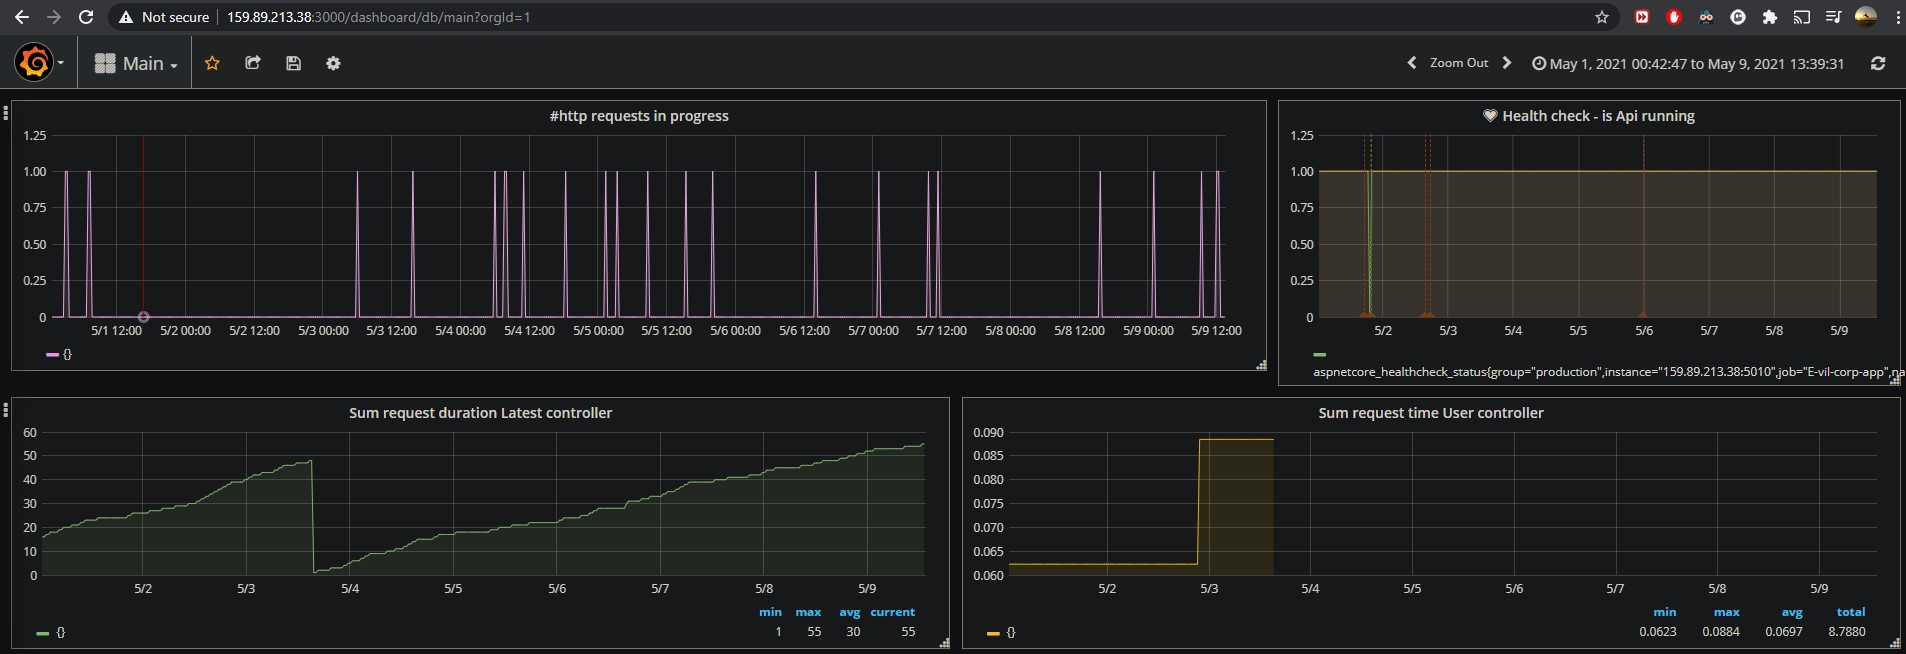
\includegraphics[width=\textwidth]{report/images/Grafana EvilTwitter 1.jpg}
                    \caption{TODO}
                    \label{fig:grafana_setup_1}
                \end{figure}
                
                \begin{figure}[H]
                    \centering
                    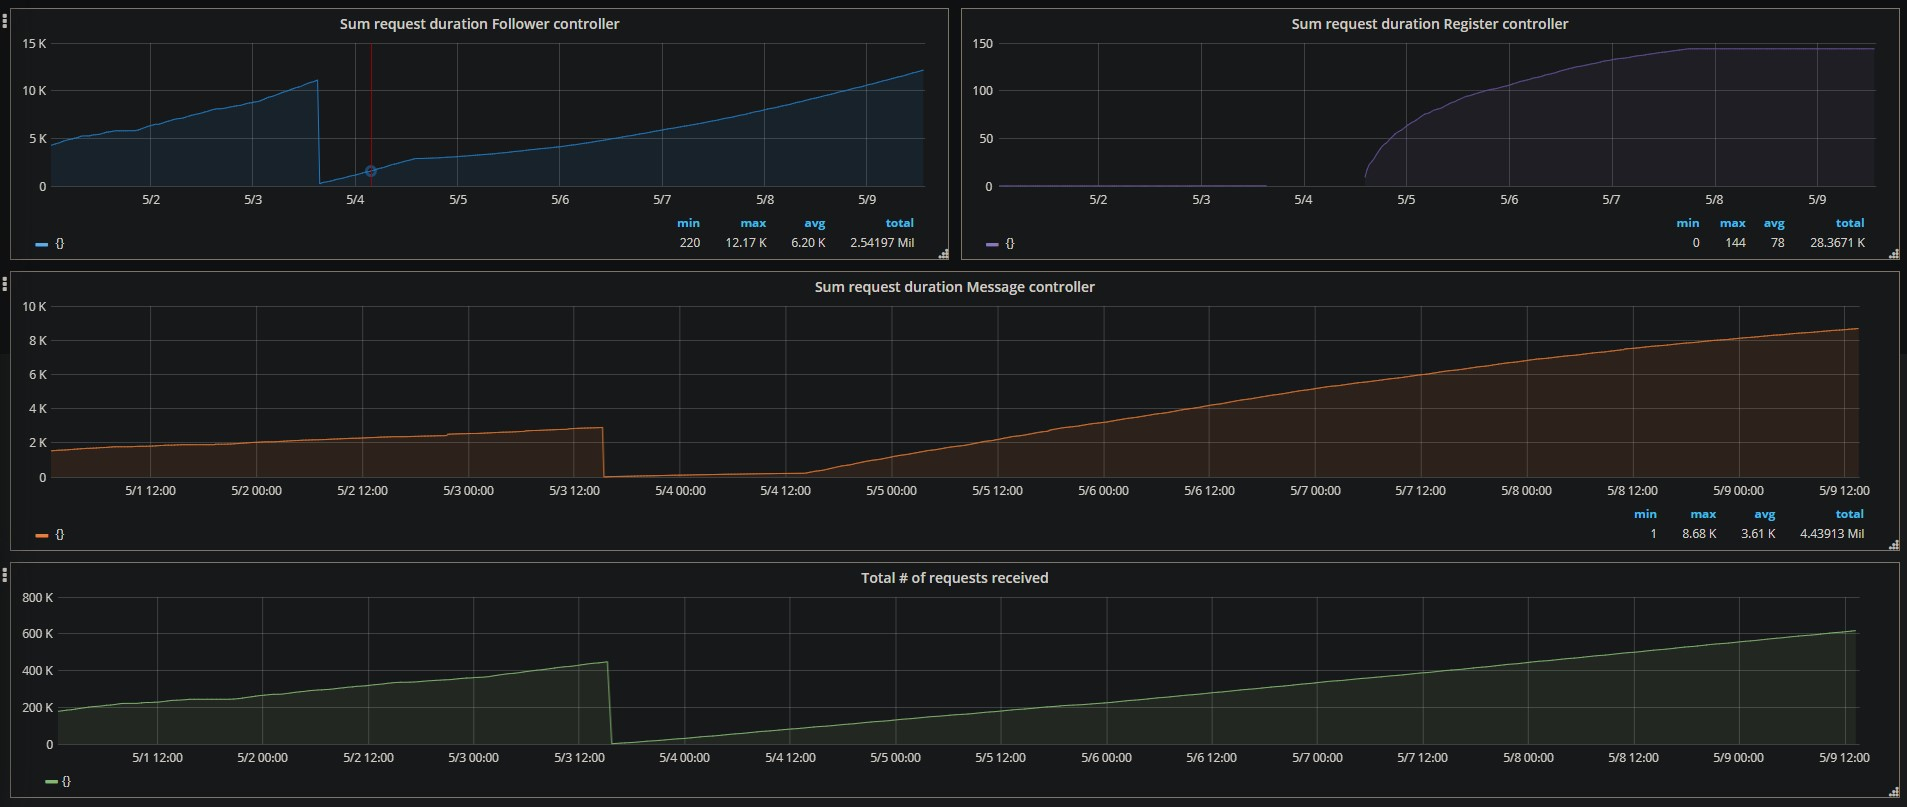
\includegraphics[width=\textwidth]{report/images/Grafana EvilTwitter 2.jpg}
                    \caption{TODO}
                    \label{fig:grafana_setup_2}
                \end{figure}
            
                First at the top row of figure \ref{fig:grafana_setup_1} the genral view of the application is given. This includes a graph over how many request is occurring at a given time (the graph to the left), to give an overview of the incoming traffic. Further, the alert graph can be seen at the top right, which is a value that can be either 1 or 0. This translates to what value latest returned last, with any latest value greater than 0 would resolved to a value of 1 and anything else would resolved to a value of 0. Hence if the Api is down or returns odd values this would be registered by Grafana. This tracker could be used to notify the developers if the Api behaved oddly, which was utilised by having a webhook that sends messages to a discord server as seen in the figure \ref{fig:grafana_discord_alert}.
                
                \begin{figure}[H]
                    \centering
                    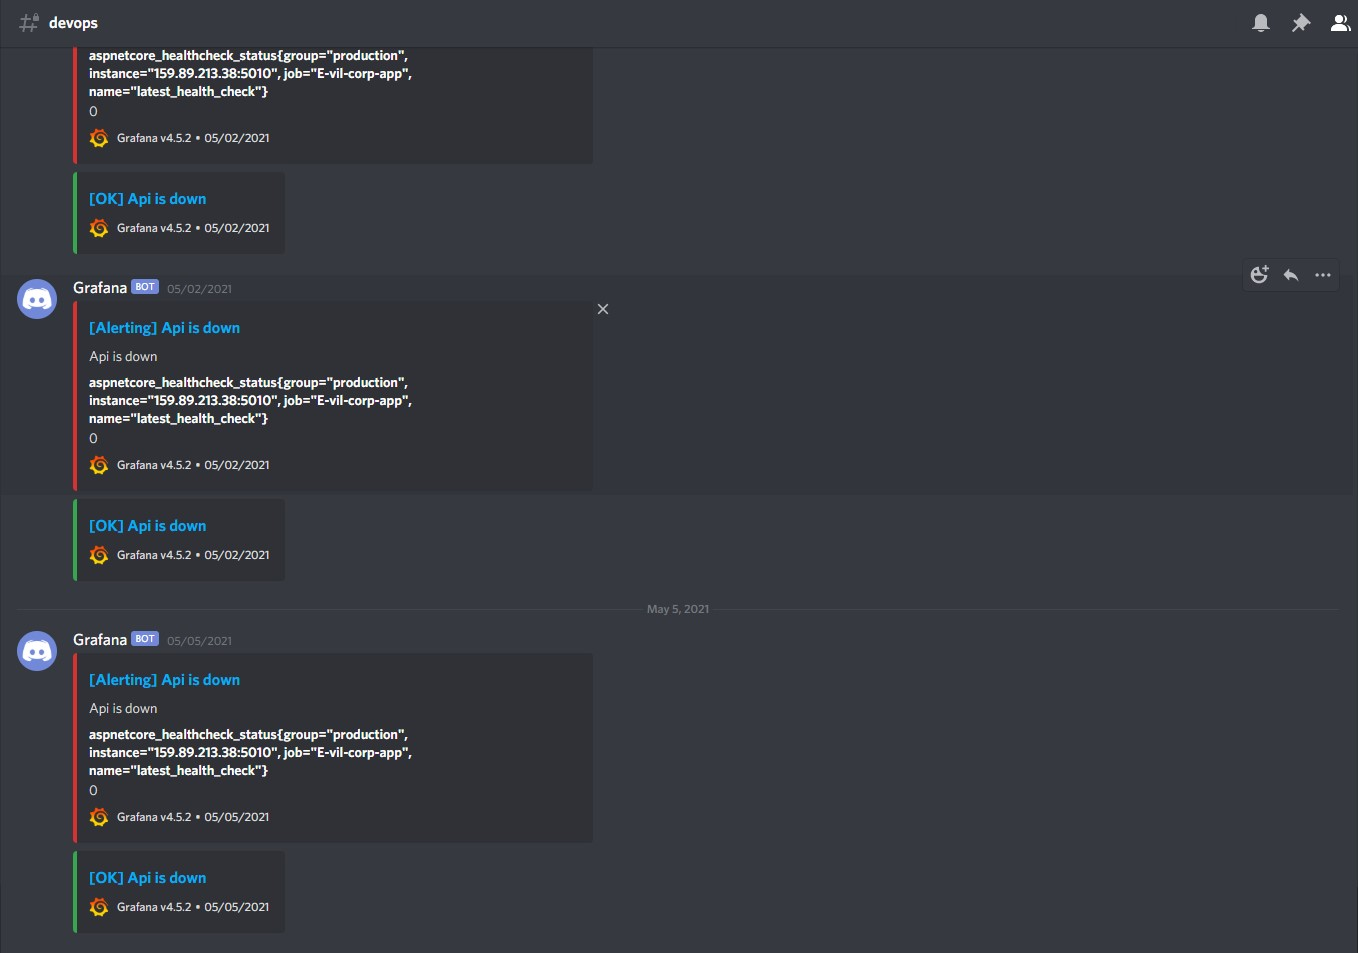
\includegraphics[width=\textwidth]{report/images/Grafana Discord Alert.jpg}
                    \caption{TODO}
                    \label{fig:grafana_discord_alert}
                \end{figure}
                
                Second information from controllers was very detailed\footnote{The data posted can be seen at \hyperlink{http://159.89.213.38:5010/metrics}{http://159.89.213.38:5010/metrics}}, and could be filtered by message type (POST, GET etc), response (204, 404 etc.). This information is valuable in solving performance issues, but creating a graph for every single message type and response would clutter the dashboard and make it less readable. Hence a decision was made that such queries should be done on a case by case basis, and a more general overview was created to monitor each controller as a whole. The query can be seen below.
                
                \begin{center}
                    sum(http\_request\_duration\_seconds\_sum{controller="Follower"})
                \end{center}
                
                Everything else on the grafana dashboard is the query above executed on all controllers. An example to the use fullness of this approach can be seen in the following example. At one point the message controller was more time as the other controllers, where by looking on the summarised time per message type revealed that it was the GET call that used a lot of time.

\end{document}